\chapter{Fundamentals of functions}
\label{ch:functions}
 
%In the capstone section, we use the activity to preview transformations, and talk about things informally. But, we don't get into any kind of $f(x)+c$ detail until we get into each of the individual families. For example, the transformations talk would first appear after we've done direct variation, and gotten into the linear forms. We focus at that time on transformations only of linear functions. Transformations of exponentials happens in the exponential unit.
%
%Note that ``big graphs'' is still there in the previous chapter, and so we'd still have informal language available about shifting up/down, steeper/shallower, wider/narrower (between big graphs and exploring the families).
%
%We save domain and range discussions until we need them. Linear functions have nothing interesting to say about domain/range, so save it. When have some more experience about how exponential equations work, the infinite progression of fractions leading to an asymptote, and how that means that there's a distinction between output values of linear and exponential functions --- then we discuss domain and range.
%
%Finally, all the ``is it a function'' stuff feels like a kind of distraction. Why is the concept so important at this very moment? I like the idea of calling things by their proper names, and if we're going to study ``functions'' we should define that term. But, I don't think we need all the detail.
%
%So, here's what I picture: A short introductory bit that defines function, gives some examples and nonexamples, but basically says: We're going to study functions in algebra 1. There are things that aren't functions, but we'll learn about those things later.
%
%I say we introduce function notation, since for the most part it's just a renaming. Plus, it gives a handy notation for evaluation.
%
%Then, I say we do the activity ``exploring the families'' (with the sorting of equations, graphs, and informal discussions of transformations) and explain the key features of each family (table, equation graph).
%
%And then we start the linear unit.
%
%Thoughts?

%A mathematician is a machine for turning coffee into theorems.
%\par\hfill --- Paul Erd\H{o}s, Hungarian mathematician

\chapquote{On two occasions I have been asked, ``Pray, Mr. Babbage, if you put into the machine wrong figures, will the right answers come out?'' I am not able rightly to apprehend the kind of confusion of ideas that could provoke such a question.}{Charles Babbage, English inventor of the first mechanical computer}

We have seen a number of relationships so far: the relationship between distance and time of a moving object, for example, or the relationship between a number's position in a sequence and that number's value. A \textit{function} is a certain kind of relationship that is of key importance to us in algebra, and indeed throughout mathematics. In this chapter we'll get an overview of functions, and then in the rest of the course we will look closely at specific kinds of functions.

% % % % % % % % % % % % % % % % % % % % % % % % % % % % % % % % % % % % % % % % 
\section{Mathematical relationships}
\label{sec:mathrelationships}

\begin{boxedexplore}[Name of Extended Exploration]
\addtodoitem{Click here to visit the extended exploration: NAME}
\end{boxedexplore}

\begin{boxedexplore}[Startup exploration: Number machines]
A number machine accepts numbers as input and produces numbers as output. When machine A receives the number 8 as input, it produces the output 28. When this machine receives $\umin12$ as input, the output is $\umin42$.

Machine B has a different mechanism for producing output values. When machine B receives the number 8 as input, it outputs 15. When it receives $\umin12$ as input, the output is $23$.

What do you suppose each machine will output when given the number $\umin7$ as input? Write a sentence explaining how you believe each machine works.
\end{boxedexplore} %% End of startup exploration

The number machines described in the startup exploration relate certain input values to certain output values. Mathematically speaking, a number machine defines a \textit{relation}.

\begin{boxeddef}[Relation]
A \gls{relation} defines how certain numbers (or other objects) are connected to other numbers (or objects). We can think of a relation as a collection of ordered pairs $(x,y)$, meaning ``$x$ is related to $y$''.
\end{boxeddef}

We might think of a number machine as a set of pairs of numbers: (input, output). Machine A in the startup exploration is defined by the pairs $(8, 28)$ and $(-12, -42)$. We sometimes say that ``machine A maps 8 to 28'' and that ``-12 is mapped to -42''.

One possible explanation is that the machine multiplies the input value by 3.5 to produce the output value. In this case, we'd expect the input $-7$ to produce the output $-24.5$. In other words, $(-7, -24.5)$ is a third point associated with machine A.

For machine B we are given the points $(8, 15)$ and $(-12, 23)$. One, somewhat complicated, explanation is that the machine doubles the input, takes the absolute value of the result, and then subtracts 1. In this case, we'd have $(-7, 13)$ as another input-output pair for machine B.\footnote{There are other rules that we could write based on the two data points we were given, and perhaps you thought of different rules than the ones we describe here. Can you find alternative explanations for how each machine works? Be creative!}

We can define relations that compare things other than numbers. For example, we might define the ``name-the-mother'' relation that accepts a person as input and which gives that person's biological mother as output. Or, we might define the ``name-the-pet'' relation, which accepts a human as input and outputs other animals.

Note that there is a difference between these two relations we have just defined. Not all people own pets, so some inputs to the name-the-pet macine have no output. Plus, some people own multiple pets, so some inputs to the name-the-pet machine have multiple outputs. On the other hand, the name-the-mother machine is guaranteed to always produce a unique output: every person has a biological mother, and every person has exactly one biological mother. It is impossible for someone to have more than one biological mother!\footnote{We don't deny that a family with two mothers is still a family! It is true that a person can have multiple mothers in a legal or emotional sense\ldots\ but a person has exactly one \textit{biological} mother.}

We saw something similar in \cref{sec:interpgraphs}, where certain graphs could be drawn in a way that would suggest an impossible situation. For example, we drew a graph (shown in \cref{fig:impossible}) that suggested Yeardleigh's submersible could at three different depths simultaneously, which -- like have more than one biological mother -- is nonsense.
%\footnote{``I like nonsense; it wakes up the brain cells.'' --- Dr. Seuss}

\begin{figure}[!htbp]
\centering
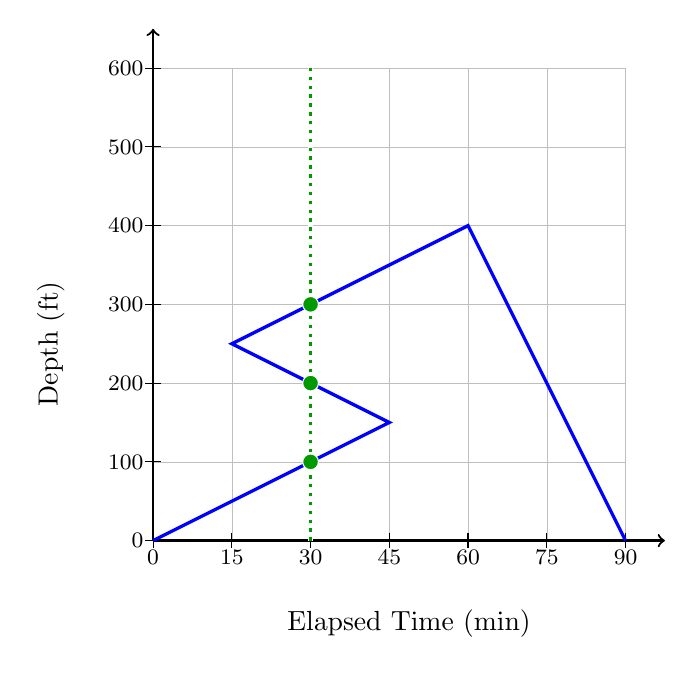
\begin{tikzpicture}[scale=1]
	\draw[ultra thin, gray!50] (0,0) grid (6,6);
	\draw[->,thick] (0,0) -- (6.5,0);
	\draw[->,thick] (0,0) -- (0,6.5);
	%% x-axis
	\foreach \x in {0,...,6}
		\draw (\x,0.1) -- (\x,-0.1);
	\foreach \x in {0,15,...,90}
		\draw (0.0667*\x, 0) node[below] {\footnotesize\x};
	\draw (3.25, -0.75) node[below] {Elapsed Time (min)};
	%% y-axis
	\foreach \y in {0,...,6}
		\draw (-0.1,\y) -- (0.1,\y);
	\foreach \y in {0,100,...,600}
		\draw (0, 0.01*\y) node[left] {\footnotesize\y};
	\draw (-1, 2.5) node[rotate=90,above] {Depth (ft)};
	%% graph
	\draw[very thick, blue] (0,0) -- (3,1.5) -- (1,2.5) -- (4,4) -- (6,0);
	\draw[ultra thick, white] (2,0) -- (2,6);
	\draw[very thick, dotted, green!60!black] (2,0) -- (2,6);
	\draw[white,fill=green!60!black] (2,1) circle[radius=0.1];
	\draw[white,fill=green!60!black] (2,2) circle[radius=0.1];
	\draw[white,fill=green!60!black] (2,3) circle[radius=0.1];
\end{tikzpicture}
	\caption{A graph of depth over time? Impossible!}
	\label{fig:impossible}
\end{figure}

Relationships that follow this very natural rule -- any given input produces a unique output -- have a special status in algebra. They're called \glspl{function}.

%From a certain point of view, there is nothing wrong with this graph --- any old squiggly line in the coordinate plane is a kind of graph. The problem arises because this graph doesn't make any sense \textit{in the context of the problem}. In this chapter, we will make some formal definitions that will help us to distinguish certain types of mathematical rules and relationships from one another.

\begin{boxeddef}[Function]
A \gls{function} is a special type of relation in which the ordered pairs have the following property: each $x$-value is paired with one, and only one, $y$-value.
\end{boxeddef}

The ``one and only one'' requirement is what makes a function special. The graph in \cref{fig:impossible} violates this requirement: certain $x$-values have more than one associated $y$-value (look at $x$ values between 15 and 45 minutes). So, this graph does not depict a function. Any given sequence is a function, since each $x$ value (position in the sequence) is occupied by exactly one $y$ value.

A sequence is a function: it would be silly to suggest that a sequence had more than one value as its third term. Depending on how we think about number machines, we might expect that a machine would act predictably and always produce the same output for a given input. A number machine that behaves in this way defines a function.

\subsubsection{Representing relations}

Ther are several ways to represent a mathematical relation. We might represent a relation using:
\begin{itemize}
\item A graph. This representation gives is a visual of the relationship between input values and output values.
\item A table of values. This representation gives us an organized list of input values and their corresponding output values. (Related forms include a \textit{mapping diagram}, or just a collection of ordered pairs.)
\item An equation. This representation gives us a rule for turning input values into output values, the way a number machine might do.
%-- A mapping diagram. Like a table, gives a series of input and corresponding output values.
%-- A set of points. Like a table, but organized differently
\end{itemize}

Since functions hold a special position in the universe of all relations, our first task is to determine whether a given mathematical relationship is, in fact, a function. To do this we have to check it against the definition of what it means to be a function. In other words, we must make sure each $x$-value corresponds to one and only one $y$-value.

%There are different features we can look for depending on the representation of the function, but the key question is always the same: does every $x$ correspond to a unique $y$?

\subsection{Graphs of functions}

In order for a graph to be a function it must avoid the situation in which multiple $y$-values stack up above a particular $x$-value. A handy way of remembering this requirement is that the graph of a function passes the \gls{vertical line test}. The vertical line test states that for the graph of a function, any vertical line drawn on the graph will intersect the graph \textit{exactly once}.

\begin{boxedex}
Which of the graphs below, if any, represents a function? How do you know?

% Graph 1
\begin{minipage}{0.33\textwidth}
\centering
Graph A
\par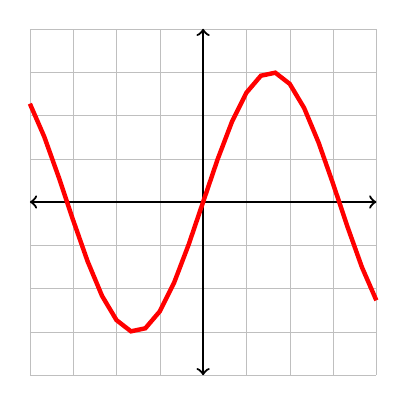
\begin{tikzpicture}[scale=0.55]
	\draw[ultra thin, gray!50] (-4,-4) grid (4,4);
	\draw[<->,thick] (-4,0) -- (4,0);
	\draw[<->,thick] (0,-4) -- (0,4);
%	\draw (0, 4.75) node {Graph A};
	%% graph
	\draw[ultra thick, red, domain=-4:4] plot (\x, {3*sin(\x r)});
\end{tikzpicture}
\end{minipage}
% Graph 2
\begin{minipage}{0.33\textwidth}
\centering
Graph B
\par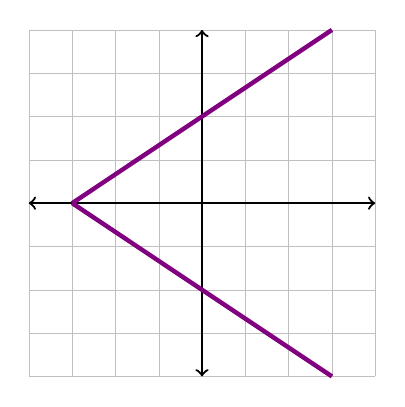
\begin{tikzpicture}[scale=0.55]
	\draw[ultra thin, gray!50] (-4,-4) grid (4,4);
	\draw[<->,thick] (-4,0) -- (4,0);
	\draw[<->,thick] (0,-4) -- (0,4);
%	\draw (0, 4.75) node {Graph B};
	%% graph
	\draw[ultra thick, violet, domain=-3:3] plot (\x,0.667*\x+2);
	\draw[ultra thick, violet, domain=-3:3] plot (\x,-0.667*\x-2);
\end{tikzpicture}
\end{minipage}
% Graph 3
\begin{minipage}{0.33\textwidth}
\centering
Graph C
\par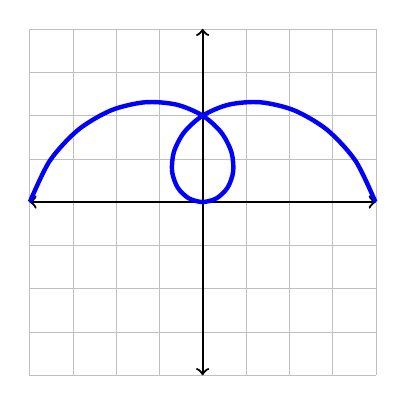
\begin{tikzpicture}[scale=0.55]
	\draw[ultra thin, gray!50] (-4,-4) grid (4,4);
	\draw[<->,thick] (-4,0) -- (4,0);
	\draw[<->,thick] (0,-4) -- (0,4);
%	\draw (0, 4.75) node {Graph C};
	%% graph
	%\draw[ultra thick, blue] (0,0) circle[radius=3cm];
	\draw[ultra thick, blue, scale=1.27,domain=-3.141:3.141,smooth,variable=\t] plot ({\t*cos(\t r)},{\t*sin(\t r)});
\end{tikzpicture}
\end{minipage}

\exsoln\ Only graph A represents a function. We can draw vertical lines on graphs B and C which intersect the graph at more than one point. This means that those $x$-values have more than one $y$-value, violating the definition of function.
\end{boxedex}

Note that in graph C, certain sections of the graph pass the vertical line test. There is no partial credit, though. A graph fails the vertical line test if any vertical line (even just one) crosses the graph in more than one point. This happens also with the graph in \cref{fig:impossible}. That graph fails the vertical line test for some vertical lines. Therefore the relationship depicted is not a function.

\begin{boxedex}
Which of the scatter plots below, if any, represents a function? How do you know? You may have to look closely!

% Graph 1
\begin{minipage}{0.33\textwidth}
\centering
Plot A
\par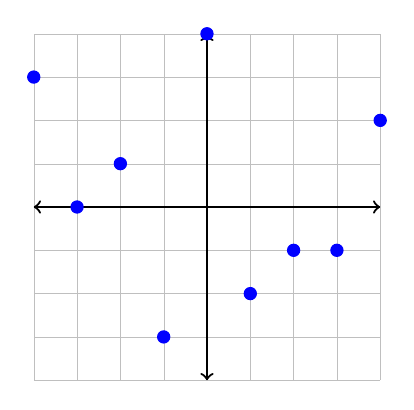
\begin{tikzpicture}[scale=0.55]
	\draw[ultra thin, gray!50] (-4,-4) grid (4,4);
	\draw[<->,thick] (-4,0) -- (4,0);
	\draw[<->,thick] (0,-4) -- (0,4);
%	\draw (0, 4.75) node {Plot A};
	%% graph
	\draw[blue] plot[only marks, mark=*, mark size=4] coordinates {(-4,3) (-3,0) (-2,1) (-1,-3) (0,4) (1,-2) (2,-1) (3,-1) (4,2)};
\end{tikzpicture}
\end{minipage}
% Graph 2
\begin{minipage}{0.33\textwidth}
\centering
Plot B
\par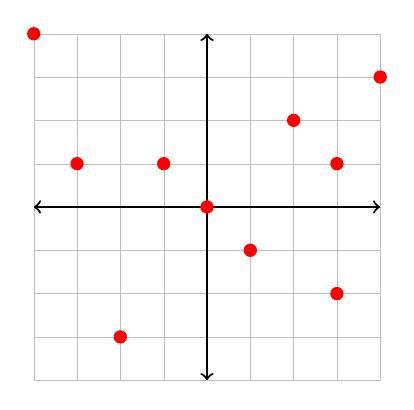
\begin{tikzpicture}[scale=0.55]
	\draw[ultra thin, gray!50] (-4,-4) grid (4,4);
	\draw[<->,thick] (-4,0) -- (4,0);
	\draw[<->,thick] (0,-4) -- (0,4);
%	\draw (0, 4.75) node {Plot B};
	%% graph
	\draw[red] plot[only marks, mark=*, mark size=4] coordinates {(-4,4) (-3,1) (-2,-3) (-1,1) (0,0) (1,-1) (2,2) (3,1) (3,-2) (4,3)};
\end{tikzpicture}
\end{minipage}
% Graph 3
\begin{minipage}{0.33\textwidth}
\centering
Plot C
\par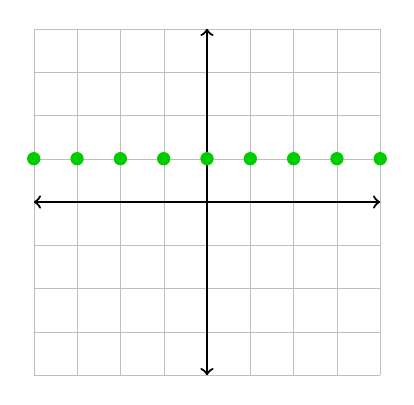
\begin{tikzpicture}[scale=0.55]
	\draw[ultra thin, gray!50] (-4,-4) grid (4,4);
	\draw[<->,thick] (-4,0) -- (4,0);
	\draw[<->,thick] (0,-4) -- (0,4);
	%% graph
	\draw[green!80!black] plot[only marks, mark=*, mark size=4] coordinates {(-4,1) (-3,1) (-2,1) (-1,1) (0,1) (1,1) (2,1) (3,1) (4,1)};
\end{tikzpicture}
\end{minipage}

\exsoln\ Plots A and C both pass the vertical line test, and therefore represent functions. Plot B fails the vertical line test because it fails for the vertical line at $x=3$.
\end{boxedex}

Note that we don't care if different $x$'s map to the same $y$. For example, in plot C, all of the $x$-values map to the same $y$-value. That's OK. In other words, a function \textit{can} fail the ``horizontal line test'' without penalty.\footnote{The horizontal line test \textit{is} a thing, and passing or failing the horizontal line test does have a mathematical meaning. But, a discussion of this will have to wait until later.}

If we think about the name-the-mother function, it is not uncommon for two different people to have the same mother: they're called siblings!

\subsection{Functions from points}

A scatter plot gives a visual representation of a collection of ordered pairs. If the ordered pairs are presented in an alternative format -- say, a table of values -- we can use the same reasoning to determine whether the given relation is a function.

\begin{boxedex}
Which of the data sets below, if any, represents a function? How do you know?

\begin{minipage}[t]{0.33\textwidth}
\centering
Set A
\par\begin{tabular}{|C{1.5cm}|C{1.5cm}|}
\hline
x & y \\\hline
-3 & 4\\
-2 & 6\\
-1 & 4\\
0 & 2\\
1 & 0\\
2 & -2\\
3 & 0\\\hline
\end{tabular}
\end{minipage}
% Graph 2
\begin{minipage}[t]{0.33\textwidth}
\centering
Set B
\par\begin{tabular}{|C{1.5cm}|C{1.5cm}|}
\hline
x & y \\\hline
2 & 1\\
1 & 2\\
-1 & 7\\
4 & 3\\
3 & 4\\
1 & 0\\
0 & 6\\\hline
\end{tabular}
\end{minipage}
% Graph 3
\begin{minipage}[t]{0.33\textwidth}
\centering
Set C
\par$(0,4) \quad (-1,6)$
\par$(2,3) \quad (0,4)$
\par$(1,5) \quad (-2,5)$
\end{minipage}

\exsoln\ Set A is a function. There are no repeated $x$-values! Set B is not a function. The $x$-value 1 appears twice and with two different related $y$-values (0 and 2). This violates the definition of function. Set C is a function. The $x$ value 0 appears twice, but it is mapped to the same value in both cases.
\end{boxedex}

A \gls{mapping diagram} is a similar way of representing a relationship between specific input and output values. Here we draw two regions (represented by a box or an oval). In one region, we list the input values, in the other region we list the output values. Then we draw arrows to show which input maps to which output.

\begin{boxedex}
Which of the mapping diagrams below, if any, represents a function? How do you know?

\begin{minipage}{0.5\textwidth}
\centering
Diagram A
\par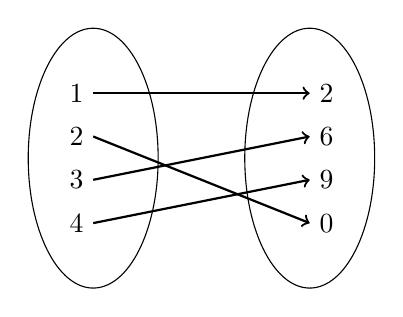
\begin{tikzpicture}[scale=0.55]
	\draw (0,0) circle[x radius=1.5, y radius=3];
	\draw (5,0) circle[x radius=1.5, y radius=3];
	\draw (0, 1.5) node[left]{1};
	\draw (0, 0.5) node[left]{2};
	\draw (0, -0.5) node[left]{3};
	\draw (0, -1.5) node[left]{4};
	\draw (5, 1.5) node[right]{2};
	\draw (5, 0.5) node[right]{6};
	\draw (5, -0.5) node[right]{9};
	\draw (5, -1.5) node[right]{0};
	\draw[thick,->] (0,1.5) -- (5,1.5);
	\draw[thick,->] (0,0.5) -- (5,-1.5);
	\draw[thick,->] (0,-0.5) -- (5,0.5);
	\draw[thick,->] (0,-1.5) -- (5,-0.5);
\end{tikzpicture}
\end{minipage}
% Graph 2
\begin{minipage}{0.5\textwidth}
\centering
Diagram B
\par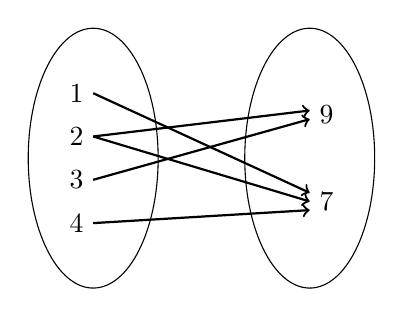
\begin{tikzpicture}[scale=0.55]
	\draw (0,0) circle[x radius=1.5, y radius=3];
	\draw (5,0) circle[x radius=1.5, y radius=3];
	\draw (0, 1.5) node[left]{1};
	\draw (0, 0.5) node[left]{2};
	\draw (0, -0.5) node[left]{3};
	\draw (0, -1.5) node[left]{4};
	\draw (5, 1) node[right]{9};
	\draw (5, -1) node[right]{7};
	\draw[thick,->] (0,1.5) -- (5,-0.8);
	\draw[thick,->] (0,0.5) -- (5,1.1);
	\draw[thick,->] (0,0.5) -- (5,-1);
	\draw[thick,->] (0,-0.5) -- (5,0.9);
	\draw[thick,->] (0,-1.5) -- (5,-1.2);
\end{tikzpicture}
\end{minipage}

\exsoln\ The first mapping is a function. Each $x$-value maps to exactly one $y$-value. The second mapping is not a function: the value 2 maps to both 7 and 9.
\end{boxedex}

Note again that the problem in diagram 2 is \textit{not} that multiple arrows point to each of the output numbers. It's OK for multiple arrows to go \textit{toward} a certain output value. The problem is that the input value 2 has multiple arrows \textit{leaving} and going to different targets.

%The table, the mapping diagram, and the list of points are all basically the same sort of representation: we are presented with a finite number of ordered pairs. So, these representations only give a limited picture of how the function operates. The preferred representations are the graph and the equation.

% If you are given one of the others, you will likely have to convert it to a graph or an equation.

\subsection{Equations of functions}

The ``number machine'' metaphor is often helpful when thinking about a function. A number (an $x$-value) goes into the machine, the machine's rule works on the number, and another number comes out of the machine (the $y$-value). Most of the time, when we have a particular rule and a particular input, we get a single, predictable output.

For example, the equation $y = 3x$ defines a function. We can substitute in 5 for $x$. The function machine multiplies 5 by 3 and outputs 15. This generates the ordered pair $(5, 15)$ and we say that ``5 maps to 15''. If we choose other values of $x$, we can generate more ordered pairs.

Not every equation defines a function, though. In order to be a function, every input value must produce one and only one output value. In algebra 2 we will study many interesting and important mathematical relationships that are not functions. We will learn, for instance, how to write the equation for a circle -- and a circle is not a function. (Can you explain why not?)

Our focus in algebra 1, though, will be on three main ``families'' of functions, and our rules will all be of the form ``$y$ equals some expression in terms of $x$''.

%In addition to being able to determine if a relation is a function, one has to be able to convert between the different representations. We will spend more time on this when we study each family of functions in depth.

\subsection{Function notation}

%\begin{boxedexplore}[Name of Extended Exploration]
%\addtodoitem{Click here to visit the extended exploration: NAME}
%\end{boxedexplore}
%
%\begin{boxedexplore}[Name of Startup Exploration]
%Description of startup exploration.
%\end{boxedexplore} %% End of startup exploration

We can thank Swiss mathematician Leonhard Euler for the concept of a function.\footnote{The surname Euler is German, and so it is pronounced $OIL \cdot er$ (and \textit{not} $YOO \cdot ler$).} He was the first to coin the term ``function'' and was the first to use a handy way of writing a function, called \textit{function notation}.

Up until now, we have used ``$y=$ something in terms of $x$'' to define all of our rules. Euler's function notation looks a bit different, but it is quite helpful in certain situations. The generic form of function notation is ``$f(x)~=$ something in terms of $x$''. In this case, we simply replace $y$ with the notation $f(x)$, which is read aloud as ``$f$ of $x$'' or ``$f$ as a function of $x$''.

In its generic form, the letter $f$ is used to name the function. We use the letter $f$, of course, because it stands for ``function''. And as usual, we use $x$ to represent the independent variable.

What's nice about this notation is that it allows us great flexibility to use other letters or symbols that can be more descriptive. For example, if we wanted to describe how the height of a bouncing ball changes over time, we might want to let the variable $t$ represent time, and then name the function $h$ for height.

So, we could write a function ``$h(t) =$ some expression in terms of $t$''. That's read ``$h$ of $t$'', which does a pretty good job of capturing the idea that we're describing \textit{height} in terms \textit{of time}.

We might write a function like $d(t) = 60t$ which described distance traveled $d$ as a function of time $t$. This is exactly the same equation as $y = 60x$, but we've changed the names of things to better match the context.

\subsubsection{Evaluation using function notation}

Function notation has another convenience. We can use the notation to indicate a specific choice of value for the independent variable. Earlier, we said: ``Evaluate the function $y = x^2-4$ when $x = 3$.'' This was fine, but function notation gives us a way to shorten these instructions.

For example, if we have $f(x) = x^2-4$ then we might want to evaluate $f(3)$, which is said aloud ``$f$ of three''. The $x$ in the function notation was replaced by 3, which is exactly what is means to evaluate the function at that value! The notation is telling us to input 3 for $x$ and find the output value. So if $f(x) = x^2 - 4$, then \[f(3) = (3)^2 - 4 = 9 - 4 = 5.\]

We will use function notation and $y =$ notation through this course. The flexibility of function notation means that it is the preferred way of writing functions in higher level mathematics courses.


% % % % % % % % % % % % % % % % % % % % % % % % % % % % % % % % % % % % % % % 
\section{Domain and range}

%\begin{boxedexplore}[Name of Extended Exploration]
%\addtodoitem{Click here to visit the extended exploration: NAME}
%\end{boxedexplore}

Machines (meaning real, mechanical devices) are physical things that have physical limitations. Number machines (meaning functions) often have similar operational restrictions.

\begin{boxedexplore}[Startup exploration: The ins and outs of functions]
Consider the function machines below.
\[f(x) = \abs{x} \qquad\qquad g(x)=\frac{1}{x}\]
% \qquad\qquad h(x)=\frac{3}{x-2}\]
What sorts of values are allowed as input to each of these machines? What sorts of values will each one produce as output?
\end{boxedexplore} %% End of startup exploration

A blender is a machine that has limited operating parameters. Anything we put into the blender comes out ``blended'' in some way. But, of course, there are some things we can't put in a blender: a piano, for example.\footnote{We'll pause here to note that ``blended'' is defined rather loosely: smoothies come out ``blended'', ice comes out ``crushed'', chickpeas come out ``pur\'eed'', magazines come out ``shredded''\ldots\ We consider all of these to be a kind of ``blended''. Speaking of magazines, we'll also mention that there are things which one \textit{can} put into a blender, but \textit{shouldn't}.} Similarly, we wouldn't put bread into a  blender, hit the button, and expect toast to pop out. That kind of output is associated with a different machine.

\subsection{Regarding input values}

An important component of the definition of any function is a specification about what sorts of numbers it can accept as input. In the language of mathematics, we call the set of all ``legal'' input values the \textit{domain} of the function.

\begin{boxeddef}[Domain]
The set of all allowed input values to a function. This is the set of all allowed $x$-values, or all possible values of the independent variable.
\end{boxeddef}

We have two functions in the startup exploration. The first function, $f(x)=\abs{x}$, is very welcoming: any real number can be used as unput to this number machine: whole numbers, fractions, positive numbers, negative numbers, it doesn't matter. The other function is a little more finicky.

In \cref{ch:numbers}, we discussed the illegality of division by zero. So, if we try to put 0 into the function $g(x)=\frac{1}{x}$, then we're going to have a problem: $g(0)$ -- that's the function $g$ evaluated at $x=0$ -- is undefined. So, our user manual for the function $g$ has to include a note that only numbers other than 0 are allowed as input. We say that the function $g(x)$ has a \textit{limited} or \textit{restricted domain}.

%%%What does this mean for the function $h(x) = \frac{3}{x-2}$, which also has $x$ in its denominator? In this case, $h(0)$ is no problem:
%%%\[h(0) = \frac{3}{0-2} = \frac{3}{-2} = -\frac{3}{2}.\]
%%%The problem in this case is when $x=2$, for then the denominator is $2-2=0$. So, $h$ has the restriction that only numbers other than 2 are allowed as input.
%%%
%%%\subsubsection{Limited domains}
%%%
%%%We say that the function $g(x)$ has a \textit{limited} or \textit{restricted domain}. 
%%%There are certain values that cannot be allowed as input because the function would ``break''.
%%%
%%%Another function with a limited domain is the square-root function $y = \sqrt{x}$. This function can only accept nonzero numbers as input. All negative numbers are restricted from the domain.\footnote{Try to take the square root of a negative number on a calculator and see what happens! Stay tuned for more on this phenomenon, and other stuff about square roots, in \cref{ch:radicals}.}

There are other circumstances where we will want or need to limit the domain. For example, if we write an equation that shows distance as a function of time, it usually makes sense to limit the domain to only include positive time-values. So, a domain can be limited by context.

A sequence is a function whose domain is limited to the set of natural numbers (the positive integers). We saw this in \cref{ch:sequences,,ch:graphs}: a sequence can have a first term and a second term, but no one-and-a-halfth term. We exclude from the domain of a sequence all numbers except $1, 2, 3, 4, \dotsc$.

We can also define a specific domain for convenience. On an assignment, for example, we might be asked to evaluate the function $y=4x+5$ for the $x$-vales $-1$, 0, and 1. We did something like this in \cref{ex:evaluating}. This is another example of limiting the domain.

%%%The three families of functions that we will study most closely in algebra 1 (the linear, exponential, and quadratic families) do not require any domain restrictions, which is good news.

\subsection{Regarding output values}

In addition to knowing about input values, it is often important for us to know what sorts of numbers we can expect as output from a certain function. We call the set of all output values the \textit{range} of the function.

\begin{boxeddef}[Range]
The set of all output values from a function. This is the set of all $y$-values, or all possible values of the dependent variable.
\end{boxeddef}

The function $f(x) = \abs{x}$ can accept any number as input, but only non-negative numbers ever come out. We say that the range of $f$ is non-negative real numbers.

In the case of $g(x) = \frac{1}{x}$, notice that the only way for a fraction to equal 0 is if the numerator is equal to zero. No matter what nonzero input value we put into the function $g$, we will never get 0 as the output! The range of $g$ is nonzero real numbers.

%%%This is also true of $h(x) = \frac{3}{x-2}$. No matter what (legal) value of $x$ we choose, $h(x)$ will never be 0. This function to has range of nonzero real numbers.

\subsubsection{Piecewise definition}

An interesting way to control the output of a function is to give it different definitions depending on the input. For example, suppose we define a function like so:
\begin{equation*}
f(x) = \begin{cases}
~x	& \text{if $x$ is positive}
\\
-x	& \text{if $x$ is negative}
\\
~0	& \text{if $x$ is equal to 0}
\end{cases}
\end{equation*}
This unusual notation gives us several definitions at once, depending on which of the ``if'' statements applies to a given input value $x$.

If the input $x$ is positive, then the output is simply $x$ itself. If the input is negative, then the output is the opposite of $x$ (so again, we get a positive value). Finally, in the third case, if the input is 0, then we get 0 as the output. Do you recognize this function? This case-by-case definition is really just a complicated way of saying $f(x) = \abs{x}$.

Here's a more interesting example. Suppose we define a function whose domain is the non-negative integers as follows:
\begin{equation*}
z(n) = \begin{cases}
~~\dfrac{~n~}{2} & \text{if $n$ is even}
\\[3ex]
-\dfrac{n+1}{2} & \text{if $n$ is odd}
\end{cases}
\end{equation*}
This function produces different output depending on whether the input value is even or odd. Let's try the first few input values to see what happens. What happens when we input 0? Zero is an even number, so the first case applies and:
\[z(0) = \frac{0}{2} = 0.\]
One is an odd number, so the second case applies:
\[z(1) = -\frac{1+1}{2} = -\frac{2}{2} = -1\]
Two is even, and three is odd. So we have:
\[z(2) = \frac{2}{2} = 1 \qquad\text{and}\qquad z(3) = -\frac{3+1}{2} = -\frac{4}{2} = -2.\]
This function produces the sequence:
\[0, -1, ~1, -2, ~2, -3, ~3, -4, ~4,\cdots\]
which is a list of all the integers. In other words: this machine turns the natural numbers $\N$ (plus zero) into the set of integers $\Z$.\footnote{This function suggests a shocking idea. Most people would say that there are more integers than there are natural numbers. After all, since the integers include all of the natural numbers \textit{and} all of the opposites of the natural numbers, it must be that the set of integers has \textit{twice as many members}\ldots\ right? Nope! The set of natural numbers and the set of integers are \textit{exactly the same size}. Think of it this way: the function $z$ defined above pairs up natural numbers and integers. If I give you a natural number (input), can you tell me what integer (output) it partners up with? If I give you an integer (output), can you tell me what natural number (input) it partners up with? If so, then the two sets match up exactly and neither set has any leftovers. They must therefore be the same size! Mind blown!}

%%%
%%%\subsection{Domain and range from tables and graphs}
%%%
%%%\begin{boxedex}
%%%Consider the table of values below. Does this table represent a function? If so, what are the domain and range given?
%%%
%%%\begin{center}
%%%\begin{tabular}{|C{2cm}|C{2cm}|}
%%%\hline
%%%x	& y\\\hline
%%%5	& 14\\
%%%6	& 17\\
%%%7	& 20\\
%%%8	& 23\\\hline
%%%\end{tabular}
%%%\end{center}
%%%
%%%\exsoln\ Based on the table, we do have a function since no $x$-values are repeated. To state the domain and range from a tabular representation, we just list the values in set notation. The domain is $x \in \{5, 6, 7, 8\}$, and the range is $y \in \{14, 17, 20, 23\}$.
%%%\end{boxedex}
%%%
%%% JASON SAYS NO
%%%
%%%When given a portion of a graph and asked to find domain and range, the key is to look at maximum and minimum values. Consider the below, showing a piece of a function. What can we say about its domain and range?
%%%
%%%\resizeplot{-8}{-8}{8}{8}
%%%\begin{figure}
%%%\begin{tikzpicture}
%%%	\begin{axis}[standard]
%%%		\draw[very thick, blue] (axis cs: -4,5) -- (axis cs: 6,-3);
%%%		\draw[very thick, blue, fill=white] (axis cs: -4, 5) circle[radius=0.15cm];
%%%		\draw[very thick, blue, fill=white] (axis cs: 6, -3) circle[radius=0.15cm];
%%%	\end{axis}
%%%\end{tikzpicture}
%%%\end{figure}
%%%
%%%The domain is the set all possible $x$-values. In this case, the graph spans the $x$-values between $-4$ and 6. To state this in mathematical symbols, recall the hungry alligators of your elementary school days. For example, do you recall filling in bubbles like this
%%%\[6~\text{\LARGE$\bigcirc$}~5\]
%%%with symbols like these?
%%%\begin{center}
%%%\begin{tabular}{cl}
%%%$<$	& less than\\
%%%$>$	& greater than\\
%%%$\leq$	& less than or equal to\\
%%%$\geq$	& greater than or equal to
%%%\end{tabular}
%%%\end{center}
%%%
%%%We can use these inequality symbols to describe the domain. We know that $x$ must be less than 6, and we can write this $x < 6$. We also know that $x$ must be greater than $-4$, or equivalently that $-4$ must be less than $x$. That's $-4 < x$. Together, we write:
%%%\[\text{domain: }-4 < x < 6\]
%%%to show that $x$ must be between $-4$ and 6. The range is the set of all possible $y$-values, and we can use the same reasoning to write:
%%%\[\text{range: }-3 < y < 5\]
%%%
%%%Note the open circle endpoints on the graph above. We use these to show that the enpoint itself is not included in the set we are describing. In these situations we use < and > to show that 
%%%
%%%On the other hand filled in circle endpoints are inclusive and use $\leq$ or $\geq$.
%%%
%%%
%%%
%%%
%%%Example 3
%%%
%%%Problem: State the Domain and Range
%%%
%%%Solution:
%%%This graph is pretty straight forward because it is a line.
%%%
%%%Looking along the x-axis, you will notice that the domain spans -5 to 6. The endpoint at -5 is open and the one at 6 is.
%%%
%%%Looking along the y-axis, the range spans -3 to 4. -3 is closed and 4 is open.
%%%
%%%Domain: $-5 < x \leq 6$
%%%Range: $-3 \leq y < 4$
%%%
%%%Example 4
%%%
%%%Problem: State the Domain and Range
%%%
%%%Solution:
%%%This graph is has a curve that peaks above either end points. This will affect the range as the domain is identical to that of example 3.
%%%
%%%Looking along the y-axis, the range spans -3 to 7. -3 is closed and 7 is closed.
%%%
%%%Domain: $-6< x \leq 6$
%%%Range: $-3 \leq y \leq 7$
%%%
%%%Notice that I used the exact same end points for each of the graphs. That is to show you that it is not just the end points that determine the domain and range. You have to be aware of what happens between the end points, especially for the range.
%%%
%%%
%%%
%%% % % % % % % % % % % % % % % % % % % % % % % % % % % % % % % % % % % % % % % 
%%%\section{Transformations in the plane}
%%%
%%%As we saw in \cref{sec:mathrelationships}, the graph of a function is a particularly helpful for understanding the relationship described by the function. One of the skills we'll develop as we go forward in this course is the ability to connect features of the equation of a certain function to features of its graph.
%%%
%%%Over time and with practice, we'll get better at picturing the graph of a function in our mind's eye without having to draw the graph on paper. Drawing graphs will still be informative, of course, but some features of the graph will start to ``jump out at us'' simply from looking at the rule for the function.
%%%
%%%\begin{boxedexplore}[Extended exploration: Transforming graphs]
%%%\addtodoitem{Click here to visit the extended exploration: Transforming Graphs}
%%%\end{boxedexplore}
%%%
%%%\begin{boxedexplore}[Startup exploration: Huh?]
%%%
%%%Description of startup exploration.
%%%
%%%\end{boxedexplore} %% End of startup exploration
%%%
%%%Discussion about startup exploration.
%%%
%%%\subsection{Transformations of Functions}
%%%
%%%Geometrically speaking, a transformation is any ...
%%%
%%%The key transformations are:
%%%\begin{itemize}
%%%\item \textit{Translation}: sliding a figure up, down, left, or right
%%%\item \textit{Reflection}: like in a mirror
%%%\item \textit{Dilation}: stretching or shrinking a figure
%%%\item \textit{Rotation}: Turning or twisting a figure
%%%\end{itemize}
%%%
%%%Our focus in algebra 1 is on the first three types of transformations. We won't get into rotations of functions now. They will return later in your mathematical career!
%%%
%%%\subsubsection{Translation Up or Down}
%%%
%%%The transformation $f(x) + b$ will move a graph up or down. If $b$ is positive, then the graph will move up. If $b$ is negative, then the graph will move down.
%%%
%%%\subsubsection{Translation Right or Left}
%%%
%%%The transformation $f(x -c)$ will shift a graph left or right. If $c$ is positive, the graph will be shifted to the right, if $c$ is negative, the graph will be shifted to the left.
%%%
%%%\addtodoitem{Functions: could we use f(x+c) in the exploration, and have students notice the sign thing x+c versus x-c?}
%%%
%%%\subsubsection{Reflection Through the x-axis}
%%%
%%%The transformation $-f(x)$ is a reflection through the $x$-axis.
%%%
%%%\subsubsection{Dilations}
%%%
%%%The transformation $a*f(x)$ is a dilation. If $\abs{a}$ is greater than 1, the dilation is a contraction (lines become steeper, parabolas become thinner). If $\abs{a}$ is less than 1, the dilation is an expansion (lines become less steep, parabolas become wider).
%%%
%%%\addtodoitem{Functions: Transformation section needs some graphs and examples.}
%%%

% % % % % % % % % % % % % % % % % % % % % % % % % % % % % % % % % % % % % % % 
\section{Three families of algebra 1}

The majority of algebra 1 will focus on the in-depth study of three key families of functions: the linear family, the exponential family, and the quadratic family. We've encountered each of these families before, but now it's time for a more formal introduction.

\begin{boxedexplore}[Extended exploration: Exploring the three families]
\addtodoitem{Click here to visit the extended exploration: Exploring the Three Families}
\end{boxedexplore}

\subsection{Parent functions}

For a given function to be considered a member of a certain family, it must share the characteristics of other members of that family as seen in its graph, its equation, and the patterns it exhibits in a table of values. These features are shown in their most basic form by the \textit{parent function} of each family.

The linear parent is $y=x$ and the quadratic parent is $y=x^2$. In this course, we will consider $y=2^x$ to be the parent function for the exponential family, though other choices are possible.\footnote{A more natural choice for the exponential parent is the function $y=e^x$, where $e$ is Euler's number (yes, that's the same Euler as the function notation guy). Euler's number has many important connections to the family of exponential functions, but those will have to wait until later. By the way $e$, like $\pi$, is an irrational number: $e \approx 2.\, 71828\, 18284\, 59045\, 23536\, 02875\dotso$}

\begin{figure}
\resizeplot{-10}{-10}{10}{10}
\bigskip
% Graph 1
\begin{minipage}{0.32\linewidth}
\centering
Linear Family
\\ $f(x)=x$\par\medskip
\begin{tikzpicture}
	\begin{axis}[
			fullsize,
			axis lines = middle,
			every axis/.append style={font=\tiny},
			axis line style={thick, <->},
			xlabel={$x$},
			ylabel={$y$},
			grid = both,
			grid style={gray!25},
			allminorticks,
			clip=true
		]
		%%% Graph	--- --- --- --- --- --- --- --- --- --- --- ---
		\addplot[algcurve, green!50!black, domain=-10:10]{x};
	\end{axis}
\end{tikzpicture}
%%%\begin{tikzpicture}[scale=0.45]
%%%	\draw[ultra thin, gray!50] (-5,-5) grid (5,5);
%%%	\draw[<->,thick] (-5,0) -- (5,0);
%%%	\draw[<->,thick] (0,-5) -- (0,5);
%%%	\draw[<->, ultra thick, blue, domain=-5:5] plot (\x,\x);
%%%\end{tikzpicture}
\end{minipage}
% Graph 2
\begin{minipage}{0.32\linewidth}
\centering
Exponential Family
\\ $f(x)=2^x$\par\medskip
\begin{tikzpicture}
	\begin{axis}[
			fullsize,
			axis lines = middle,
			every axis/.append style={font=\tiny},
			axis line style={thick, <->},
			xlabel={$x$},
			ylabel={$y$},
			grid = both,
			grid style={gray!25},
			allminorticks,
			clip=true
		]
		%%% Graph	--- --- --- --- --- --- --- --- --- --- --- ---
		\addplot[algcurve, green!50!black, domain=-10:3.32]{2^x};
	\end{axis}
\end{tikzpicture}
%%%\resizeplot{-5}{-1}{5}{9}
%%%\begin{tikzpicture}
%%%	\begin{axis}[defaultgrid, allminorticks, fullsize]
%%%		\addplot[algcurve, blue, domain=-5:3.15](x, 2^x);
%%%	\end{axis}
%%%\end{tikzpicture}
%%%\begin{tikzpicture}[scale=0.45]
%%%	\draw[ultra thin, gray!50] (-5,-1) grid (5,9);
%%%	\draw[<->,thick] (-5,0) -- (5,0);
%%%	\draw[<->,thick] (0,-1) -- (0,9);
%%%	\draw[<->, ultra thick, blue, domain=-5:3.15] plot (\x,2^\x);
%%%\end{tikzpicture}
\end{minipage}
% Graph 3
\begin{minipage}{0.32\linewidth}
\centering
Quadratic Family
\\ $f(x)=x^2$\par\medskip
\begin{tikzpicture}
	\begin{axis}[
			fullsize,
			axis lines = middle,
			every axis/.append style={font=\tiny},
			axis line style={thick, <->},
			xlabel={$x$},
			ylabel={$y$},
			grid = both,
			grid style={gray!25},
			allminorticks,
			clip=true
		]
		%%% Graph	--- --- --- --- --- --- --- --- --- --- --- ---
		\addplot[algcurve, green!50!black, domain=-3.15:3.15]{x^2};
	\end{axis}
\end{tikzpicture}
%%%\resizeplot{-5}{-1}{5}{9}
%%%\begin{tikzpicture}
%%%	\begin{axis}[defaultgrid, allminorticks, fullsize]
%%%		\addplot[algcurve, blue, domain=-3:3](x, x^2);
%%%	\end{axis}
%%%\end{tikzpicture}
%%%\begin{tikzpicture}[scale=0.45]
%%%	\draw[ultra thin, gray!50] (-5,-1) grid (5,9);
%%%	\draw[<->,thick] (-5,0) -- (5,0);
%%%	\draw[<->,thick] (0,-1) -- (0,9);
%%%	\draw[<->, ultra thick, blue, domain=-3:3] plot (\x,\x*\x);
%%%\end{tikzpicture}
\end{minipage}
\caption{The parent functions of the three families}
\label{fig:parents}
\end{figure}

Compare the equations for each of the parent functions: How are they the same? How are they different? Compare the graphs: How are they the same? How are they different? When presented with a new equation of graph, what features might we look for to decide which family it belongs to?

These are not the only three families of functions out there. Invent a rule or draw a graph which \textit{does not fit} into any of these three families. What makes this rule or graph different?

In \cref{sec:mathrelationships} we learned techniques for identifying whether a given relation is a function. One of our tasks going forward will be to learn techniques for distinguishing the function families from one another.


\subsection{Transforming the parents}

As we have seen many times already, a graph can be particularly helpful way to see, and therefore understand, a mathematical relationship. One of the skills we'll develop as we go forward in this course is the ability to connect features of the equation of a certain function to features of its graph.

Over time and with practice, we'll get better at picturing the graph of a function in our mind's eye without having to draw the graph on paper. Drawing graphs will still be informative, of course, but some features of the graph will start to ``jump out at us'' simply from looking at the equation of the function.

\begin{boxedexplore}[Startup exploration: Not far from the tree]
Study the three sets of animations below. Each set of images shows a way in which we can change the parent equation and produce a change in its graph.

\Cref{fig:transa} shows what happens when we multiply the parent function by a constant value. \Cref{fig:transc} shows what happens when we add a constant value to the parent. \Cref{fig:transb} shows what happens when we add a constant value to the agrument (the $x$ value) before that value is used as input to the parent function.

Study the animations, and then write a sentence or two summarizing what is happening in each case.

\textit{Note about the animations: The images will only appear animated when this PDF document is viewed using \href{http://get.adobe.com/reader/}{Adobe Reader}. Otherwise, please visit OUR WEBSITE for an interactive versions of these animations.}

\addtodoitem{Create something on the website for this. Maybe links to desmos pages w/ sliders.}
\end{boxedexplore}

\newcommand{\animscale}{0.45}
%%% Figure 1. a*f(x) animations
\begin{figure}
\begin{minipage}{0.32\linewidth}
	\centering
	\animategraphics[scale=\animscale]{6}{anim/linea}{}{}
\end{minipage}
%
\begin{minipage}{0.32\linewidth}
	\centering
	\animategraphics[scale=\animscale]{6}{anim/expoa}{}{}
\end{minipage}
%
\begin{minipage}{0.32\linewidth}
	\centering
	\animategraphics[scale=\animscale]{6}{anim/quada}{}{}
\end{minipage}
\caption{Comparing the parent function $f(x)$ with offspring ${\color{blue}a}\cdot f(x)$.}
\label{fig:transa}
\end{figure}


%%% Figure 2: f(x)+c animations
\begin{figure}
\begin{minipage}{0.32\linewidth}
	\centering
	\animategraphics[scale=\animscale]{6}{anim/linec}{}{}
\end{minipage}
%
\begin{minipage}{0.32\linewidth}
	\centering
	\animategraphics[scale=\animscale]{6}{anim/expoc}{}{}
\end{minipage}
%
\begin{minipage}{0.32\linewidth}
	\centering
	\animategraphics[scale=\animscale]{6}{anim/quadc}{}{}
\end{minipage}
\caption{Comparing the parent function $f(x)$ with offspring $f(x)+{\color{violet}c}$.}
\label{fig:transc}
\end{figure}

%%% Figure 3: f(x+b) animations
\begin{figure}
\begin{minipage}{0.32\linewidth}
	\centering
	\animategraphics[scale=\animscale]{6}{anim/lineb}{}{}
\end{minipage}
%
\begin{minipage}{0.32\linewidth}
	\centering
	\animategraphics[scale=\animscale]{6}{anim/expob}{}{}
\end{minipage}
%
\begin{minipage}{0.32\linewidth}
	\centering
	\animategraphics[scale=\animscale]{6}{anim/quadb}{}{}
\end{minipage}
\caption{Comparing the parent function $f(x)$ with offspring $f(x+{\color{red}b})$.}
\label{fig:transb}
\end{figure}


\subsection{Fundamentals of linear functions}

The first family we will study in depth is the family of linear functions. Here we summarize the key features of this family, all of which will return in future chapters.

We will learn several different forms for the equation of a linear function. The feature they all share is that the variable $x$ has no exponent, or rather the highest power of the variable $x$ is 1. For example, the parent of this family, $y = x$, is the same as $y = x^1$. That's a ``phantom 1'' there in the exponent, and we don't usually write it.

The graph of a linear function is a straight, non-vertical line. (Can you explain why we have to exclude vertical lines from this family of functions?) We sometimes also exclude horizontal lines from this family: a function of the form ``$y=$ a number'' is a horizontal line, for example $y = 6$.

Recall that arithmetic sequences are in the family of linear functions. Arithmetic sequences have a rule that involves repeatedly adding on a constant difference at each step. So, this is the feature we see in the table of a linear function: when the $x$-values increase by a fixed amount, the $y$-values increase by a (possibly different) fixed amount.

There are two key transformations of the parent function. Multiplying by a constant value, as in $y=a \cdot x$ changes the ``steepness'' of the graph. Certain $a$ values (negative ones) cause the graph to show a decreasing trend. Adding a value as in $y=x + c$ shifts the graph upwards or downwards. Viewed from a different perspective, we could also say that this shifts the graph left or right. Up-down shifts and left-right shifts look the same for a straight line. The distinction is more clear in the other families.

%%%In the extended exploration, we saw that graphing the equation $y=3x+2$ produced a graph that was steeper than $y=x$ and also shifted upwards from the origin. Generally, if take the equation $y=mx+b$ and replace $m$ and $b$ with numbers, the number $m$ controls the steepness of the line and the number $b$ controls the vertical shift.
%%%
%%%If we think of the rule $y=mx+b$ as the rule for an arithmetic sequence, we have the recursive rule ``start with $b$, add $m$ to the previous value''.
%%%
%%%In terms of a distance-time graph, this would be like moving by a fixed amount $m$ with each tick of the clock. In other words: moving at a constant speed. This gives us a good idea of why the graph is a straight line!
%%%
%%%we wrote rules of the f: In the context of our work with sequences, $m$ was the common difference and $b$ was the $a_0$ term.
%%%
%%%ne of which is generally written $y = mx + b$. To create a specific linear function, we replace $m$ and $b$ with numbers.
%%%
%%%Later, when we study linear functions we will refer to these as slopes and y-intercepts respectively.
%%%
%%%You should have also noticed from the lesson on transformations in a plane that the ``b'' in y = mx + b caused the graph to translate up or down. Also, the ``m'' changed the steepness of the line and if it is negative, it changes the line from being increasing to decreasing (reflection through the x-axis).
%%%y=x

\subsection{Fundamentals of exponential functions}

The second family of functions we will explore in this course is the exponential family. In fact, we will begin our study of this family in algebra 1, and then return to it again in algebra 2.

An exponential equation is one in which the variable $x$ appears as the exponent (hence the name). The graph of an exponential function is a smooth, curving shape that we sometimes describe as ``J-like''. This is only an approximation, though, since an exponential graph may sometimes look more like a backwards J or an upside-down J.

Exponentials have the interesting property that while they get almost vertical on one side, and almost horizontal on the other side. In other words, one side gets ``infinitely large'' while on the other side we have tinier and tinier fractions that get closer and closed to zero\ldots\ but never actually disappear! Mathematically speaking, we say that the function approaches an \gls{asymptote} at the flat horizontal portion.

Recall that geometric sequences are in the family of exponential functions. Geometric sequences have a rule that involves repeatedly multiplying by a constant ratio. This is the feature we look for in a table.

Multiplying the parent by a value, as in $y=a\cdot2^x$, changes the steepness of the graph and -- if $a$ is negative -- causes it to be reflected over the $x$-axis.

Adding a value to the parent function -- $y=2^x+c$ -- causes a shift up or down. Adding to the argument -- $y = 2^{(x+b)}$ -- gives us a shift left or right.


\subsection{Fundamentals of quadratic functions}

We will study the quadratic family last in this course. In fact, it will be our gateway into the study of techniques that will become helpful as we learn about other families and types of functions in algebra 2.

The key feature of a quadratic equation is that the highest exponent on the variable $x$ is 2. The equation may also contain an $x$ term, but that's the same as $x^1$, so the highest power of $x$ is still 2!

The graph of a quadratic function is a smooth U-like graph called a \gls{parabola}. Of course, under certain circumstances, the U opens downwards.

The transformations of the parent function are perhaps more clear with this family. Multiplying by a constant, $y=a \cdot x^2$, changes the ``steepness'' of the graph. And, in the case that $a$ is negative, controls whether the graph opens upwards or downwards.

Adding to the parent function $y=x^2+c$ produces a clear vertical shift, and adding to the argument $y=(x+b)^2$ produces a clear horizontal shift. Interestingly, the horizontal shifts appear to be ``backwards'' compared to what we might expect. Adding to the argument shifts the graph to the left, whereas subtracting from the argument (or adding a negative value) shifts the graph to the right. More on this unusual behavior later!

Recall from our study of sequences that quadratic patterns show a constant second difference. In other words, they have a recursive rule that states: ``Start with $A$, add to each previous term the members of some arithmetic sequence.'' This constant second difference will be the feature that we look for in a data table.


\subsection{Domain and range of the three families}

It's quite easy to identify the domains of the three main families of algebra 1. Linear, exponential, and quadratic functions all have ``all real numbers'' as their domain. We can always use any number as input. This is convenient!

The range of a linear function is also pretty simple: it is all real numbers. As we saw as we transformed linear functions, the a (non-horizontal) line will eventually stretch up (or down) as high (or as low) as you want to go on the $y$-axis.

The ranges for exponential and quadratic functions are a little more complicated, but we can see what is happening by examining their graphs. Notice, for example, that the graphs of the parents $y=2^x$ and $y=x^2$ never dip below the $x$-axis.

This feature of the exponential and quadratic families will always be retained, in some form, when we transform these equations. The range will always be limited by some minimum or maximum value. 

For example, the U-shaped quadratic function always has a lowest point (if the parabola opens upwards) or a highest point (if the parabola opens downwards). We will learn more about identifying and describing the maxima and minima when we get into each family in depth.


\addtodoitem{Closing Remarks of some kind, since we're venturing off into the linear unit now...}